\chapter{Design}
This chapter describes the design of our application, ... \todo{Other things than the application?}

\section{Application Design}
In \chapref{chap:intro} we explained the idea of our application and what the application should be able to do. Based on this we need the following Android activities\todo{activities/fragments /windows? Har vi et afsnit der forklarer Android komponenter? Nødvendigt?}:

\begin{description}
\item[Exhibitions list] Is the start-up activity which shows a list of exhibitions. Here you can see information about exhibitions and choose to open the exhibitions location in a map.\todo{Skal vi lige have fundet ud af om den faktisk skal gøre det}
\item[Exhibition information] Shows information about an exhibition such as name, description, and logo.
\item[Exhibition map] Shows the map of the exhibition. The map contains markers for each booth which the user can click to access information about the booth.
\item[Booth information] Shows information about a booth, such as name, description, and subscribe button.
\item[Exhibition schedule] Is a schedule for the exhibition which shows major events happening at the exhibition.
\item[Exhibition feeds] Is a list of news feeds based on the users subscriptions.
\item[Category list] Is a list of categories, e.g. hardware, software.
\end{description}\todo{Change to actual activity names when all are created.}

\subsection*{Story}
Julie opens our application \todo{insert actual app name}. She is presented with a list of exhibitions that she browse. She browses the exhibitions and reads about them, she finds a software exhibition and decides that she want to go there. She clicks the map button which shows the exhibitions location. With her smartphone she can use her built-in \ac{gps} application to drive to the exhibition. When she arrives at the exhibition she quickly notices a sign that tells her to scan an \acs{nfc} tag. She scans the \acs{nfc} tag and the system registers a new user. An activity appears asking her what categories and related booths she would like to subscribe to. She picks Microsoft and clicks continue. Now she has access to everything about the exhibition: Exhibition information, map of the exhibition, news feed based on her subscriptions, and a schedule. Julie gets a quick overview of major events in the schedule and the news feed, and then decides to go directly to a Microsoft booth. On the map she finds a Microsoft booth, clicks it, and chose to get directions to the booth. The application remembers Julie's last known location, i.e. the last \acs{nfc} tag she scanned, and generates a route from there to the booth.

\subsection*{Prototype Design}

\begin{figure}[H]
\begin{minipage}[b]{0.5\columnwidth}
\centering

\includegraphics[width=0.7\columnwidth]{img/prototype/1.png}
\caption{Start screen\label{fig:start}}
\end{minipage}
\hspace{0.5cm}
\begin{minipage}[b]{0.5\columnwidth}
\centering
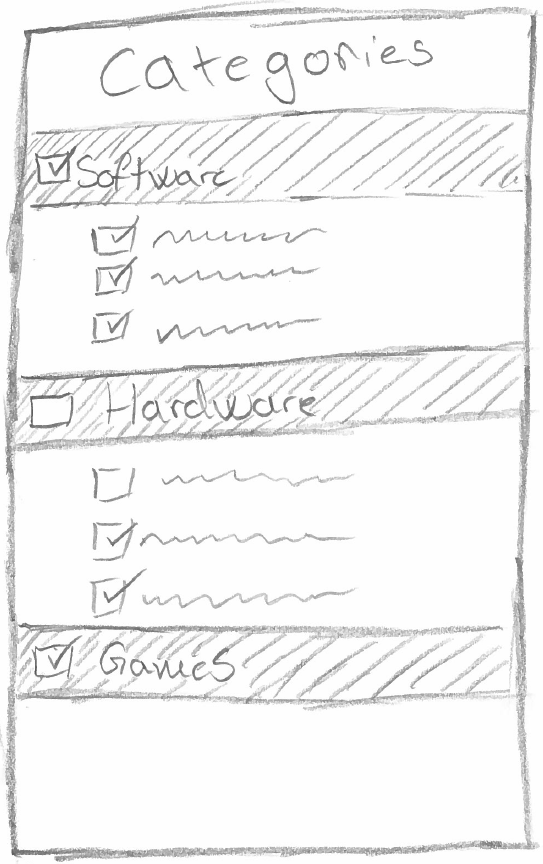
\includegraphics[width=0.7\columnwidth]{img/prototype/2.png}
\caption{Categories\label{fig:categories}}
\end{minipage}
\end{figure}

\begin{figure}[H]
\begin{minipage}[b]{0.5\columnwidth}
\centering
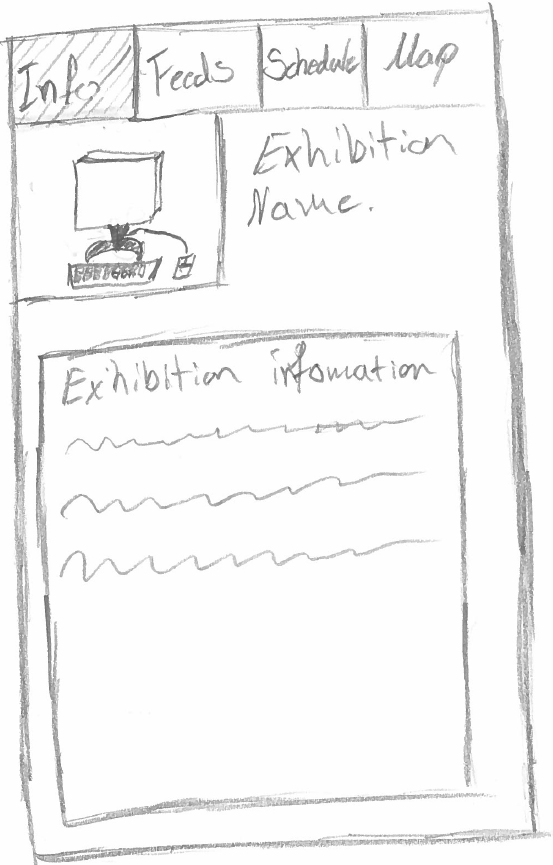
\includegraphics[width=0.7\columnwidth]{img/prototype/3.png}
\caption{Exhibition information\label{fig:exhibition}}
\end{minipage}
\hspace{0.5cm}
\begin{minipage}[b]{0.5\columnwidth}
\centering
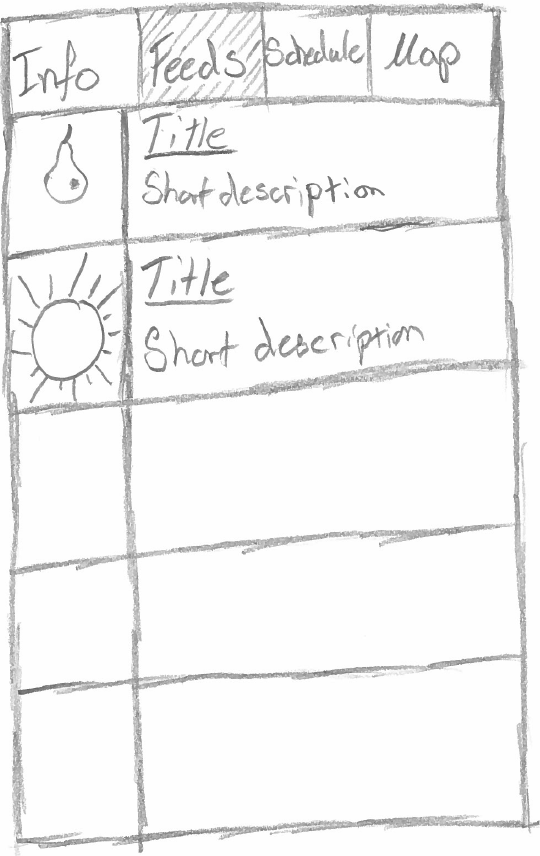
\includegraphics[width=0.7\columnwidth]{img/prototype/4.png}
\caption{Feed list\label{fig:feedlist}}
\end{minipage}
\end{figure}

\begin{figure}[H]
\begin{minipage}[b]{0.5\columnwidth}
\centering
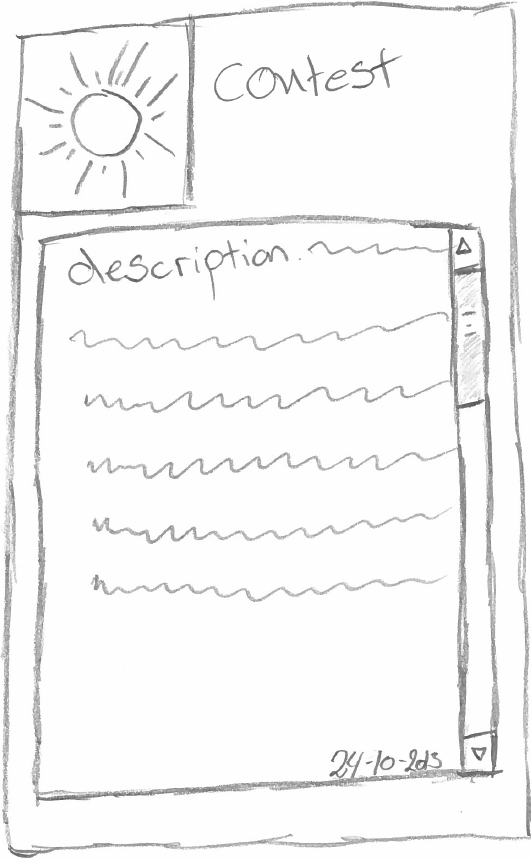
\includegraphics[width=0.7\columnwidth]{img/prototype/5.png}
\caption{Feed item\label{fig:feeditem}}
\end{minipage}
\hspace{0.5cm}
\begin{minipage}[b]{0.5\columnwidth}
\centering
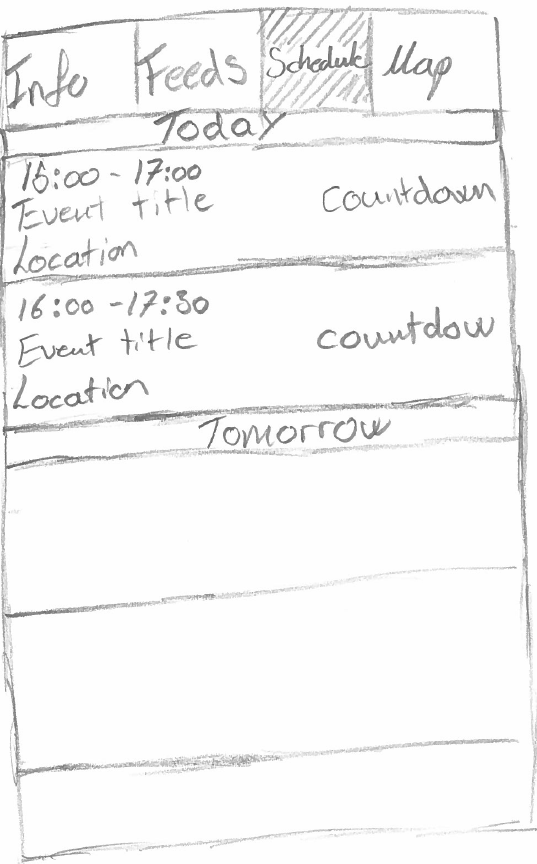
\includegraphics[width=0.7\columnwidth]{img/prototype/6.png}
\caption{Schedule\label{fig:schedule}}
\end{minipage}
\end{figure}

\begin{figure}[H]
\begin{minipage}[b]{0.5\columnwidth}
\centering
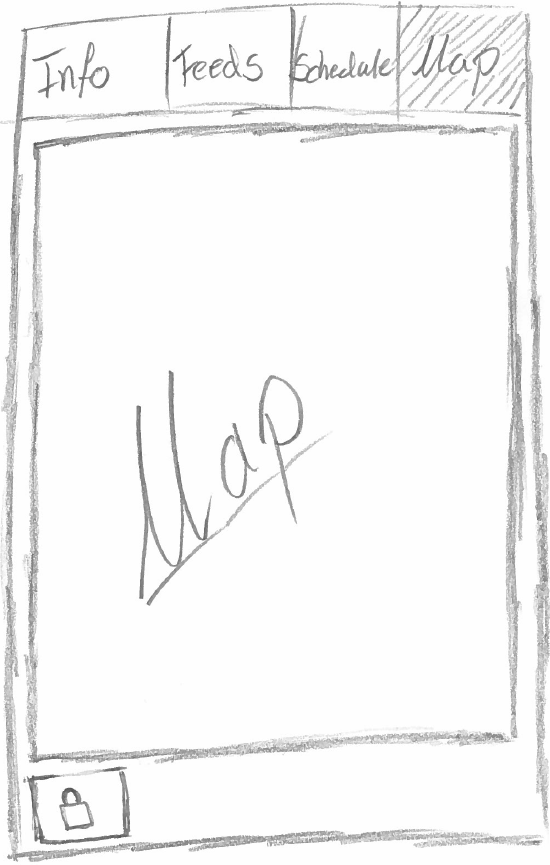
\includegraphics[width=0.7\columnwidth]{img/prototype/7.png}
\caption{Map\label{fig:map}}
\end{minipage}
\hspace{0.5cm}
\begin{minipage}[b]{0.5\columnwidth}
\centering
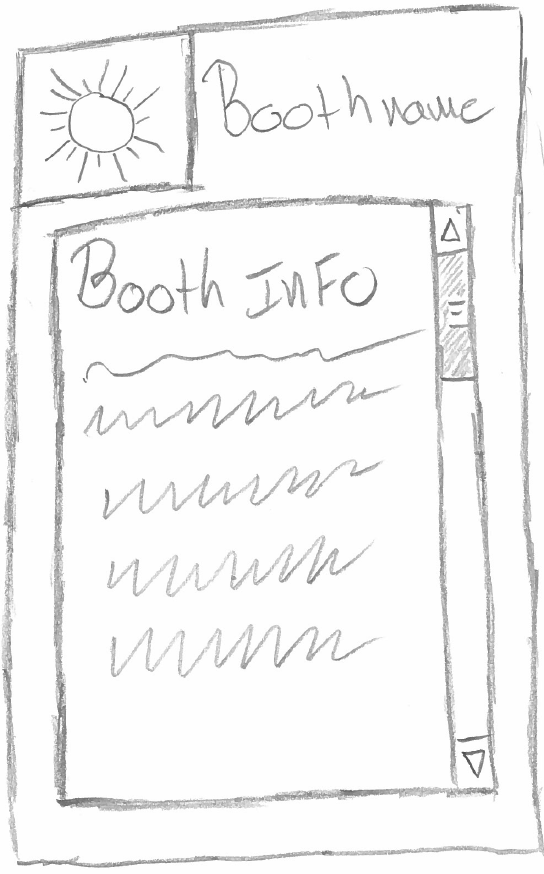
\includegraphics[width=0.7\columnwidth]{img/prototype/8.png}
\caption{Booth information\label{fig:booth}}
\end{minipage}
\end{figure}

\pagebreak
\section{Final Application Design}
\todo{Pictures and description of the finished application}

\begin{figure}[H]
\begin{minipage}[b]{0.5\columnwidth}
\centering
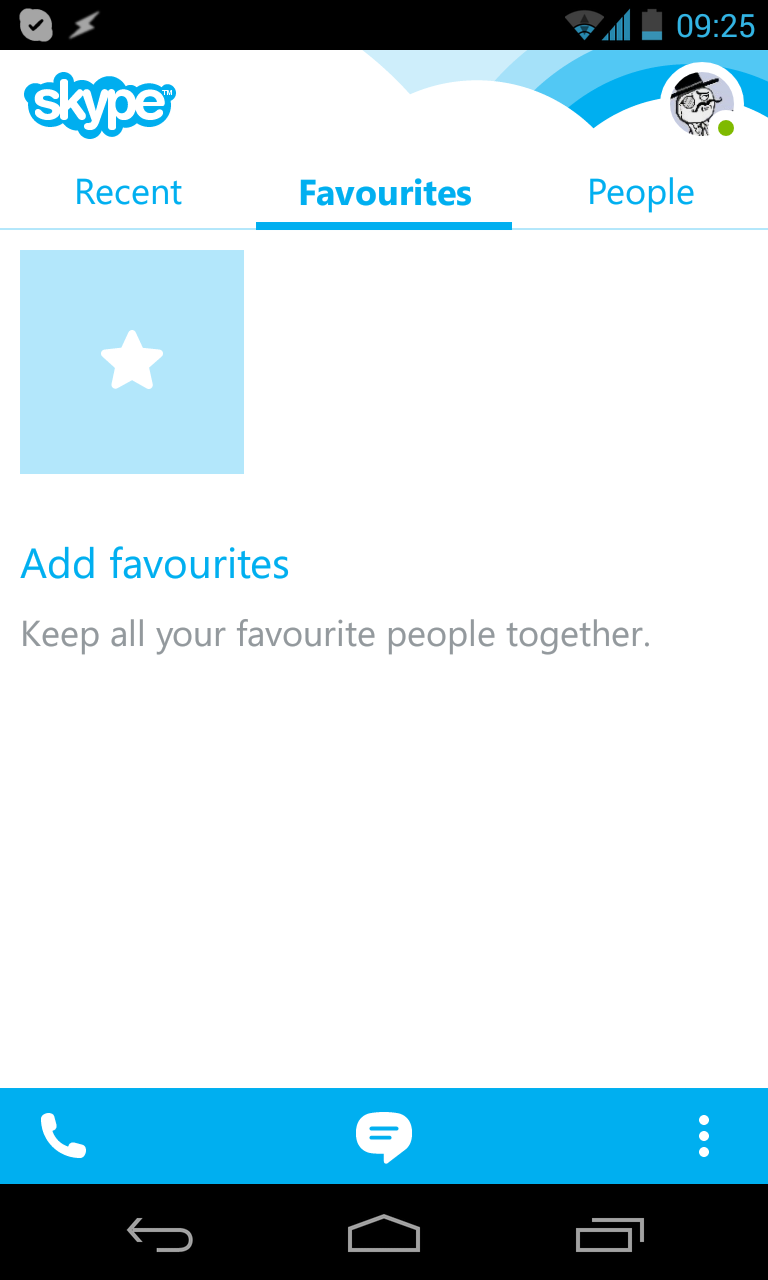
\includegraphics[width=0.7\columnwidth]{img/screenshots/twitter.png}
\caption{Skype\label{fig:skype}}
\end{minipage}
\hspace{0.5cm}
\begin{minipage}[b]{0.5\columnwidth}
\centering
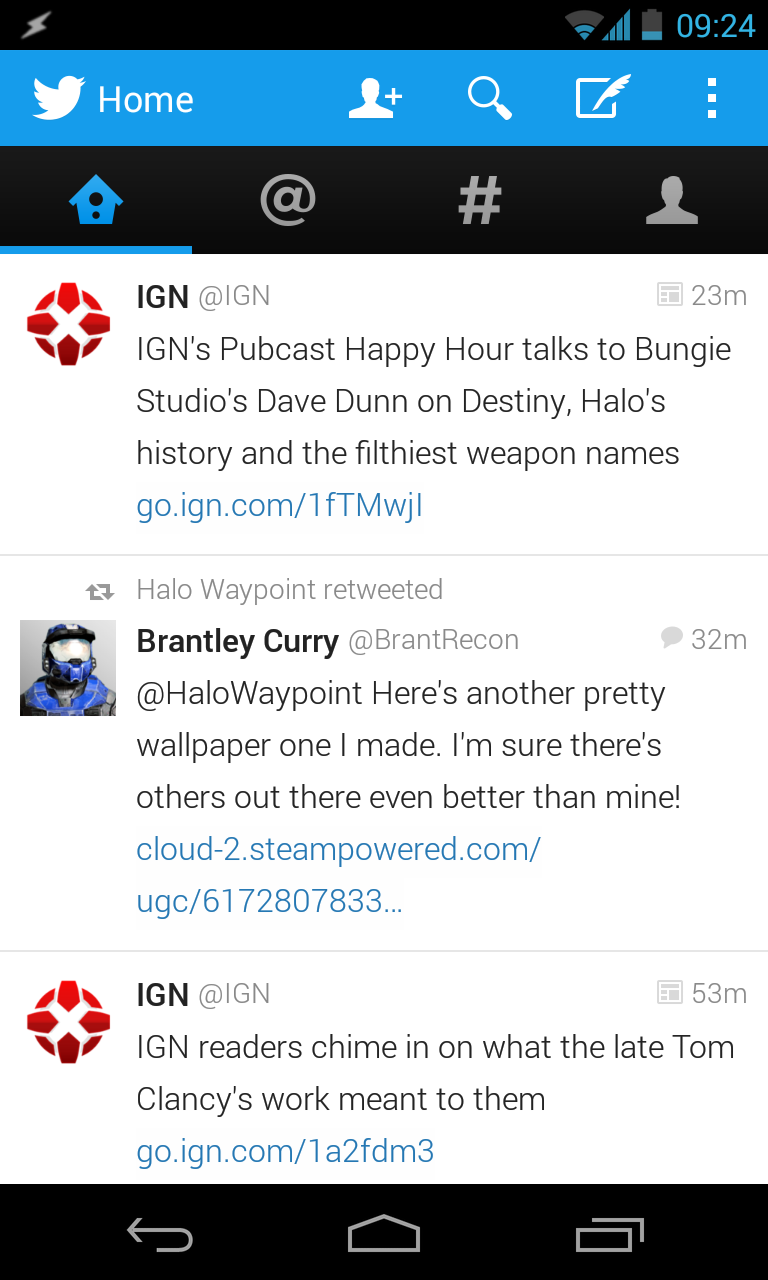
\includegraphics[width=0.7\columnwidth]{img/screenshots/skype.png}
\caption{Twitter\label{fig:twitter}}
\end{minipage}
\end{figure}

Before designing our our application we looked at a few other applications to get inspiration for our design.

We decided that using tabs, like Skype in  \autoref{fig:skype}, was a good way for the user to easily see multiple activities by just swiping to the side.

We recognised that we were going to create a few different lists for the application, for this we looked at Twitter \autoref{fig:twitter} and tried to capture their simplicity of tweets in our list items.\todo{Måske nævne at vi tog udgangspunkt i Twitter for feeds.}